% Type of the document
\documentclass{beamer}

% elementary packages:
\usepackage{graphicx}
\usepackage[latin1]{inputenc}
\usepackage[T1]{fontenc}
\usepackage[english]{babel}
\usepackage{listings}
\usepackage{xcolor}
\usepackage{eso-pic}
\usepackage{mathrsfs}
\usepackage{url}
\usepackage{amssymb}
\usepackage{amsmath}
\usepackage{multirow}
\usepackage{hyperref}
\usepackage{booktabs}
\usepackage{multicol}

% additional packages
\usepackage{bbm}

% packages supplied with ise-beamer:
\usepackage{cooltooltips}
\usepackage{colordef}
\usepackage{beamerdefs}
\usepackage{lvblisting}

% Change the pictures here:
% logobig and logosmall are the internal names for the pictures: do not modify them. 
% Pictures must be supplied as JPEG, PNG or, to be preferred, PDF
\pgfdeclareimage[height=2cm]{logobig}{hulogo}
% Supply the correct logo for your class and change the file name to "logo". The logo will appear in the lower
% right corner:


% Title page outline:
% use this number to modify the scaling of the headline on title page
\renewcommand{\titlescale}{1.0}
% the title page has two columns, the following two values determine the percentage each one should get
\renewcommand{\titlescale}{1.0}
\renewcommand{\leftcol}{0.6}

% Define the title.Don't forget to insert an abbreviation instead 
% of "title for footer". It will appear in the lower left corner:
\title[Predictive Analytics: Credit Scoring]{Predictive Analysis of Customer Credit Data }
% Define the authors:
\authora{Yousuf Hasan Siddiqui} % a-c
\authorb{Orhan Ipek}
\authorc{Shikhar Srivastava}

% Define any internet addresses, if you want to display them on the title page:
%\def\linka{http://lvb.wiwi.hu-berlin.de}
\def\linkb{}
\def\linkc{}
% Define the institute:
\institute{Statistical Programming Language \\
Humboldt--Universit�t zu Berlin \\}

% Comment the following command, if you don't want, that the pdf file starts in full screen mode:
\hypersetup{pdfpagemode=FullScreen}

%Start of the document
\begin{document}

% create the title slide, layout controlled in beamerdefs.sty and the foregoing specifications
\frame[plain]{
\titlepage
}

% The titles of the different sections of you talk, can be included via the \section command. The title will be displayed in the upper left corner. To indicate a new section, repeat the \section command with, of course, another section title
%%%%%%%%%%%%%%%%%%%%%%%%%%%%%%%%%%%%%%%%%%%%%%%%%%%%%%%%%%%%%%%%%%%%%%%%%%%%%%%%%%%%%%%%%%%%%%%%%%%%%%%%%%%%%%%%%%%%%%%%
\section{Introduction}
%%%%%%%%%%%%%%%%%%%%%%%%%%%%%%%%%%%%%%%%%%%%%%%%%%%%%%%%%%%%%%%%%%%%%%%%%%%%%%%%%%%%%%%%%%%%%%%%%%%%%%%%%%%%%%%%%%%%%%%%

\frame{
\frametitle{Outline}

\begin{enumerate}
\item Introduction 
\item Motivation
\item Data Set
\item Descriptive Statistics
\item Encoding Data
\item Predictive Modelling
\item Results
\end{enumerate}
}

%%%%%%%%%%%%%%%%%%%%%%%%%%%%%%%%%%%%%%%%%%%%%%%%%%%%%%%%%%%%%%%%%%%%%%%%%%%%%%%%%%%%%%%%%%%%%%%%%%%%%%%%%%%%%%%%%%%%%%%%
\section{Background and Importance}
%%%%%%%%%%%%%%%%%%%%%%%%%%%%%%%%%%%%%%%%%%%%%%%%%%%%%%%%%%%%%%%%%%%%%%%%%%%%%%%%%%%%%%%%%%%%%%%%%%%%%%%%%%%%%%%%%%%%%%%%

% Subsections are not visible on the actual slide, but are displayed as bookmarks in the pdf file. Their application facilitates an easy navigation trough large pdf files.
%%%%%%%%%%%%%%%%%%%%%%%%%%%%%%%%%%%%%%%%%%%%%%%%%%%%%%%%%%%%%%%%%%%%%%%%%%%%%%%%%%%%%%%%%%%%%%%%%%%%%%%%%%%%%%%%%%%%%%%%
\subsection{General ideas}
%%%%%%%%%%%%%%%%%%%%%%%%%%%%%%%%%%%%%%%%%%%%%%%%%%%%%%%%%%%%%%%%%%%%%%%%%%%%%%%%%%%%%%%%%%%%%%%%%%%%%%%%%%%%%%%%%%%%%%%%

%%%%%%%%%%%%%%%%%%%%%%%%%%%%%%%%%%%%%%%%%%%%%%%%%%%%%%%%%%%%%%%%%%%%%%%%%%%%%%%%%%%%%%%%%%%%%%%%%%%%%%%%%%%%%%%%%%%%%%%%
\frame{
\frametitle{Introduction}

\begin{itemize}
\item Constantly increasing outstanding consumer loans is one of the biggest problems in financial industry.
\begin{figure}
	\begin{center}
	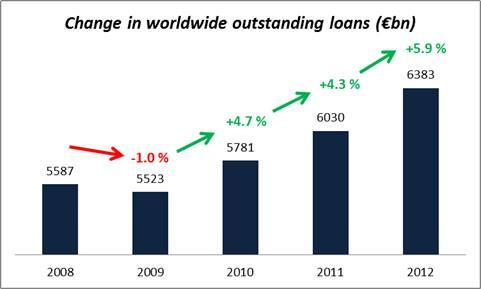
\includegraphics[scale=0.3]{Figures/loandata}
	\caption{Sources: Central banks, Aster�s, Cr�dit Agrole} 
	\end{center}
\end{figure}
\item The credit approval decision involves the manual categorization of customers using various scoring and risks calculations.
\end{itemize}
}

%%%%%%%%%%%%%%%%%%%%%%%%%%%%%%%%%%%%%%%%%%%%%%%%%%%%%%%%%%%%%%%%%%%%%%%%%%%%%%%%%%%%%%%%%%%%%%%%%%%%%%%%%%%%%%%%%%%%%%%%
%%%%%%%%%%%%%%%%%%%%%%%%%%%%%%%%%%%%%%%%%%%%%%%%%%%%%%%%%%%%%%%%%%%%%%%%%%%%%%%%%%%%%%%%%%%%%%%%%%%%%%%%%%%%%%%%%%%%%%%%
\frame[containsverbatim]{
\frametitle{Motivation}

\begin{itemize}
\item  Improvement in the computing machines and machine learning algorithms are swiftly adopted by the financial sector.
\item Predictive analytics gives us the opportunity to use vast amounts of data to find trends and patterns and make future predictions. 
\item Efficient and rapid decision process
\item Using machine learning helps as the algorithm updates itself without extra need of parameter calculation.  
\end{itemize}
}


%%%%%%%%%%%%%%%%%%%%%%%%%%%%%%%%%%%%%%%%%%%%%%%%%%%%%%%%%%%%%%%%%%%%%%%%%%%%%%%%%%%%%%%%%%%%%%%%%%%%%%%%%%%%%%%%%%%%%%%%
\frame[containsverbatim]{
\frametitle{Data Set}

\begin{itemize}
\item German Credit Data
\item Mixture of Quantitative and Qualitative Attributes
\item Observations: 1000 , Variables: 20
\item Data Features:
	\begin{itemize}
	\item No missing values
	\item Outliers
	\end{itemize}
\end{itemize}
}


%%%%%%%%%%%%%%%%%%%%%%%%%%%%%%%%%%%%%%%%%%%%%%%%%%%%%%%%%%%%%%%%%%%%%%%%%%%%%%%%%%%%%%%%%%%%%%%%%%%%%%%%%%%%%%%%%%%%%%%%
\section{Descripitive Statistics}
%%%%%%%%%%%%%%%%%%%%%%%%%%%%%%%%%%%%%%%%%%%%%%%%%%%%%%%%%%%%%%%%%%%%%%%%%%%%%%%%%%%%%%%%%%%%%%%%%%%%%%%%%%%%%%%%%%%%%%%%

\frame[containsverbatim]{
\frametitle{Overview}
\begin{itemize}
\item Understand and describe data at an aggregate level
\item Qualitative Variables
	\begin{itemize}
	\item Bar Plots
	\item Mosaic Plots
	\end{itemize}

\item Quantitave Variables
    \begin{itemize}
	\item Histograms
	\item Kernel Plots
	\item Box Plots
	\end{itemize}

\end{itemize}

}

%%%%%%%%%%%%%%%%%%%%%%%%%%%%%%%%%%%%%%%%%%%%%%%%%%%%%%%%%%%%%%%%%%%%%%%%%%%%%%%%%%%%%%%%%%%%%%%%%%%%%%%%%%%%%%%%%%%%%%%%

%%%%%%%%%%%%%%%%%%%%%%%%%%%%%%%%%%%%%%%%%%%%%%%%%%%%%%%%%%%%%%%%%%%%%%%%%%%%%%%%%%%%%%%%%%%%%%%%%%%%%%%%%%%%%%%%%%%%%%%%

\frame{
\frametitle{Bar Plots}
\begin{figure}[htb]
	\begin{center}
	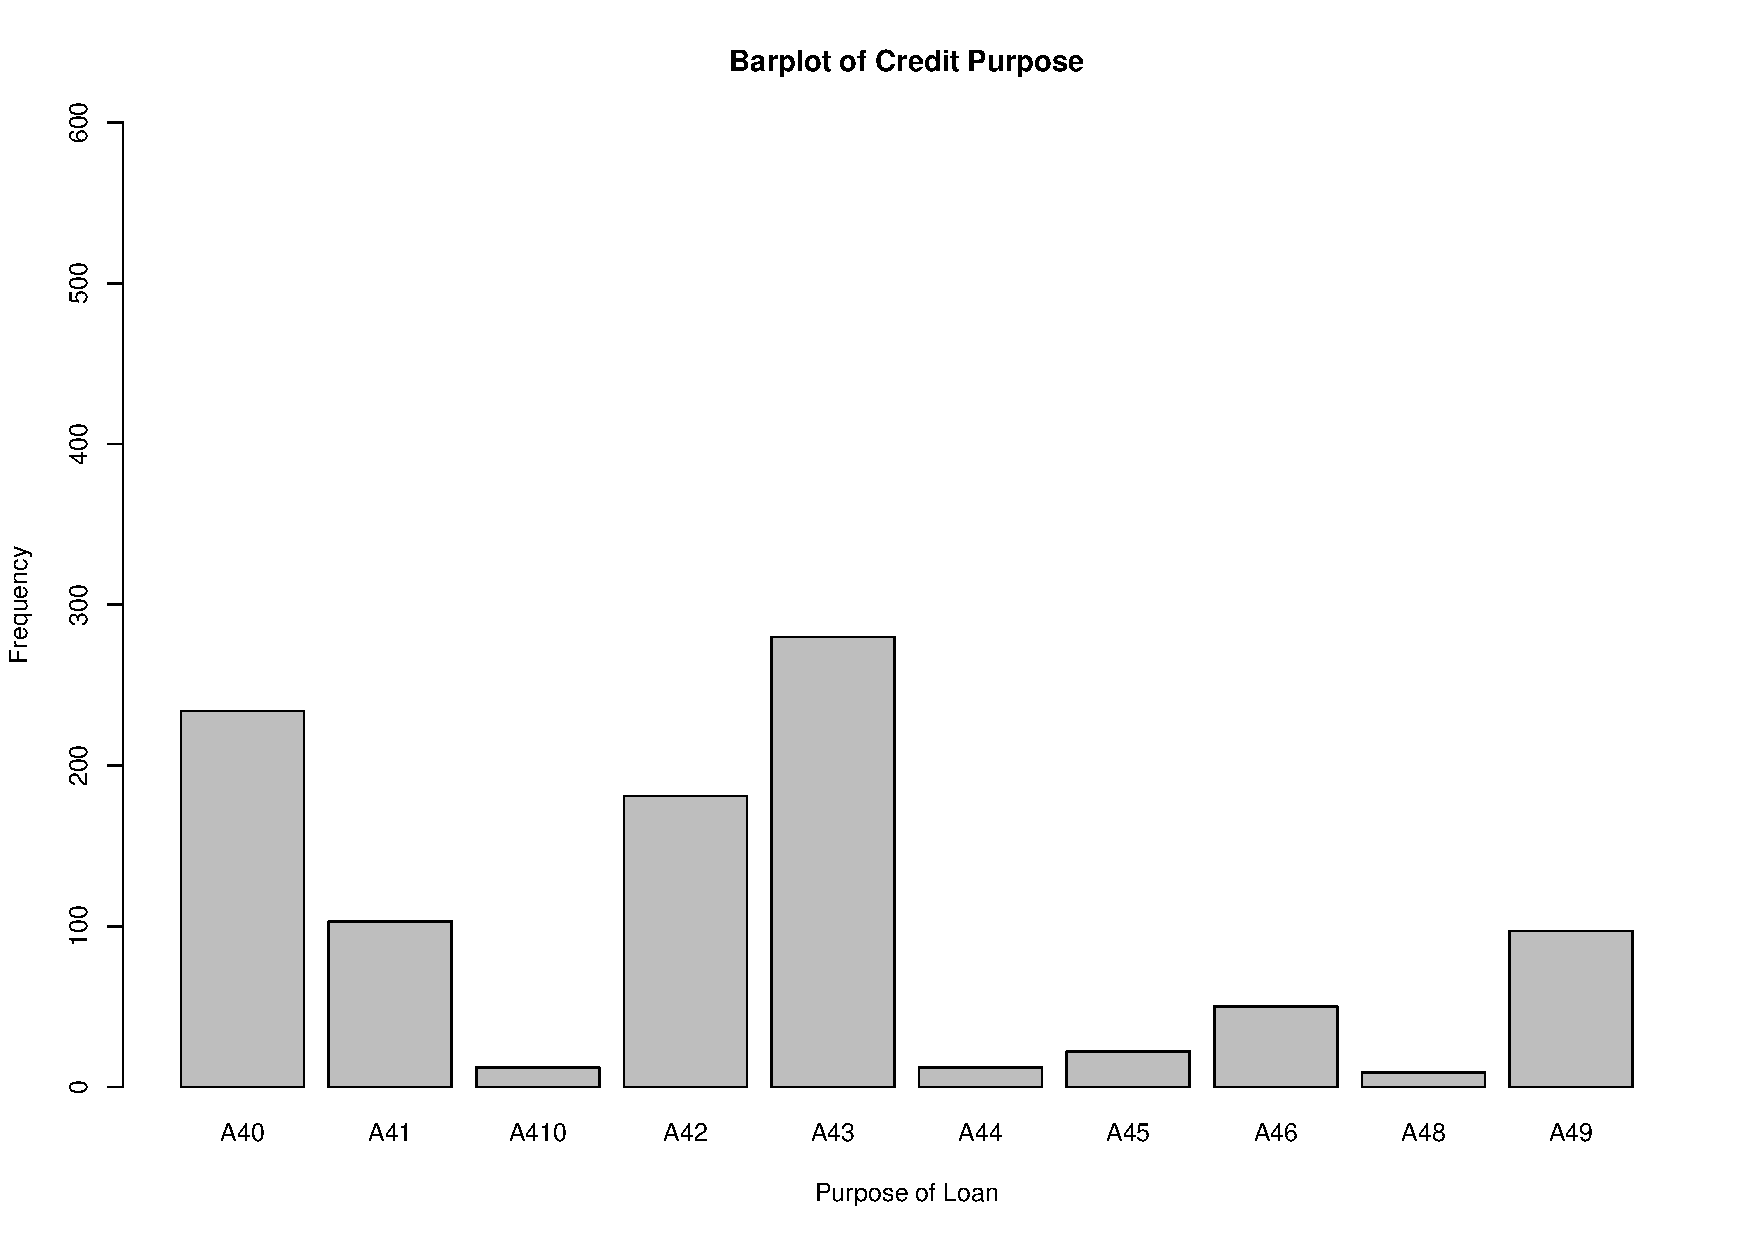
\includegraphics[scale=0.3]{Figures/barplot_credit_purpose}	
	\end{center}
\end{figure}

}

%%%%%%%%%%%%%%%%%%%%%%%%%%%%%%%%%%%%%%%%%%%%%%%%%%%%%%%%%%%%%%%%%%%%%%%%%%%%%%%%%%%%%%%%%%%%%%%%%%%%%%%%%%%%%%%%%%%%%%%%

\frame{
\frametitle{Bar Plots}
\begin{figure}[htb]
	\begin{center}
	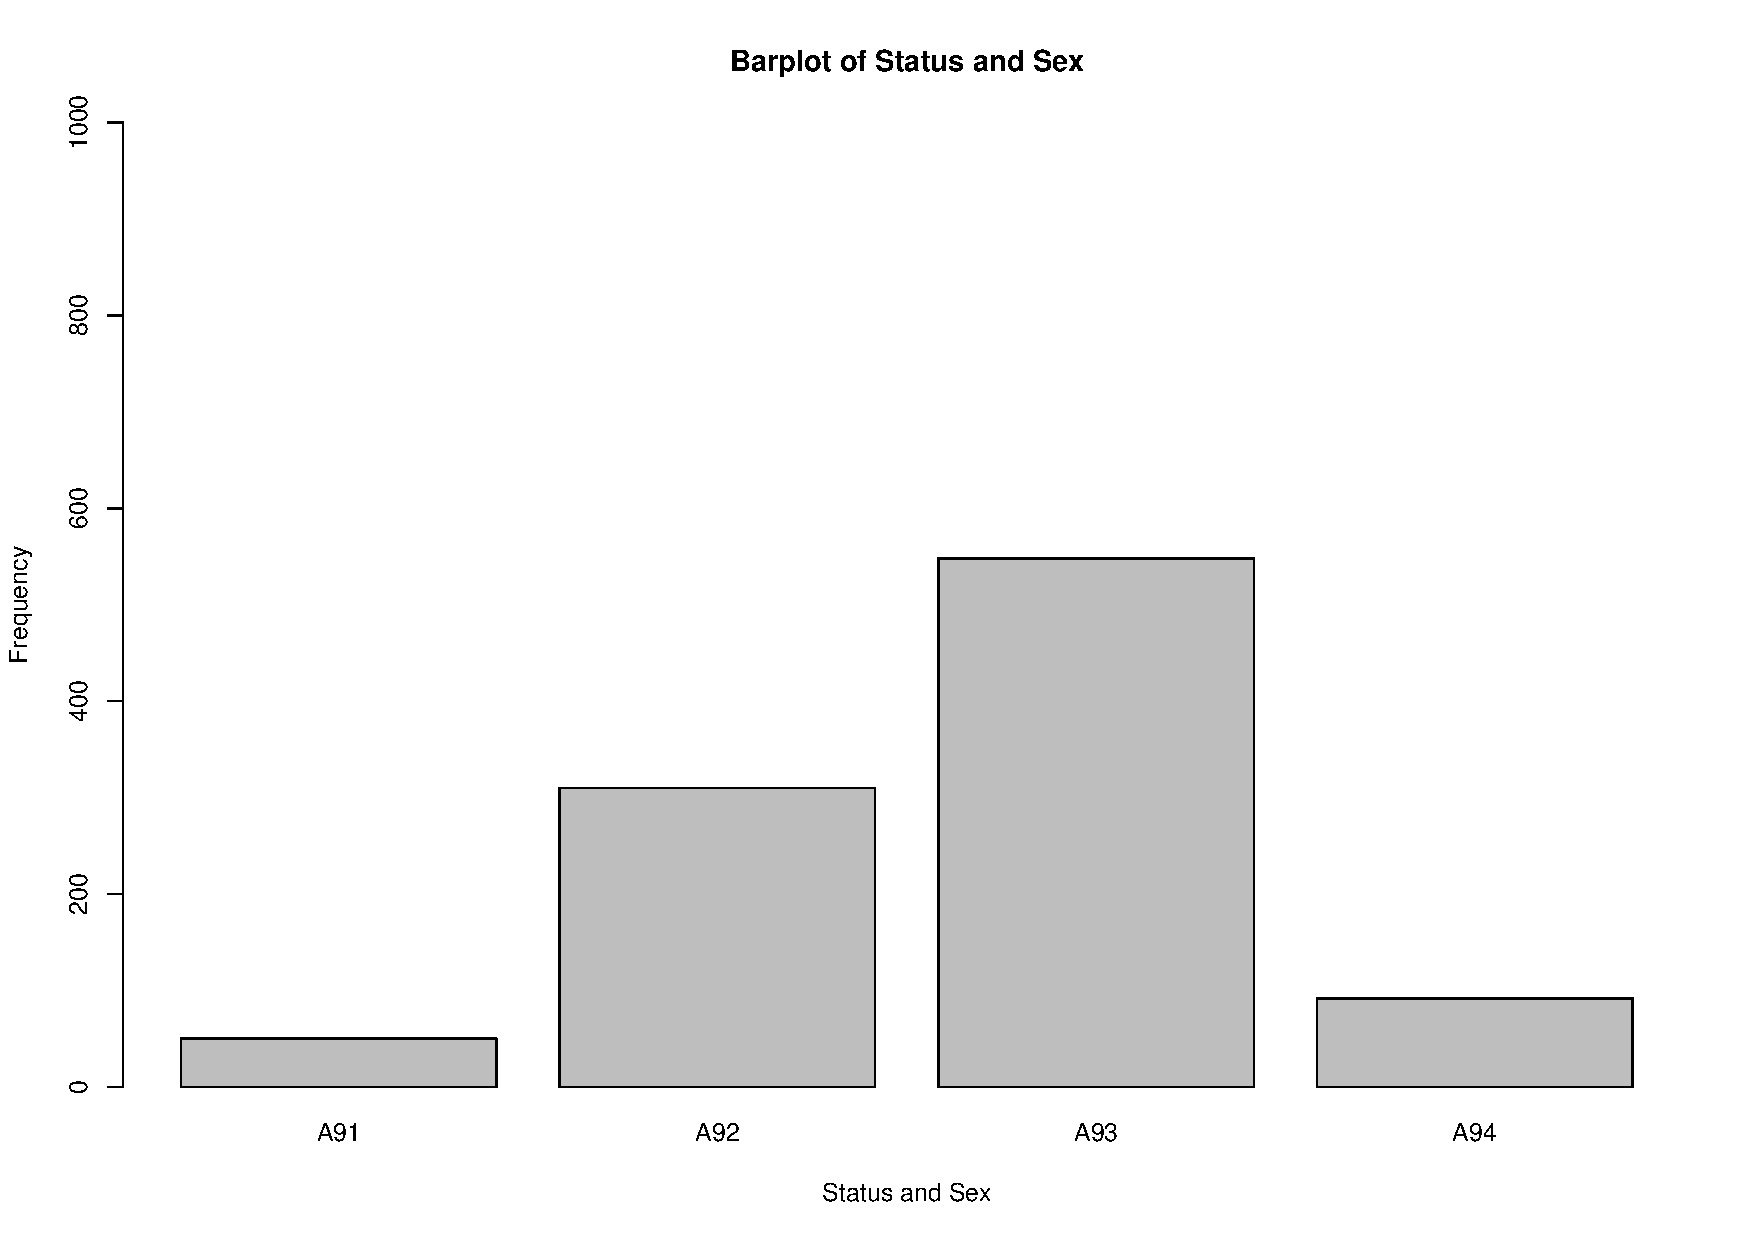
\includegraphics[scale=0.3]{Figures/barplot_status_and_sex}	
	\end{center}
\end{figure}

}

\frame{
\frametitle{Mosaic Plots}
\begin{figure}[htb]
	\begin{center}
	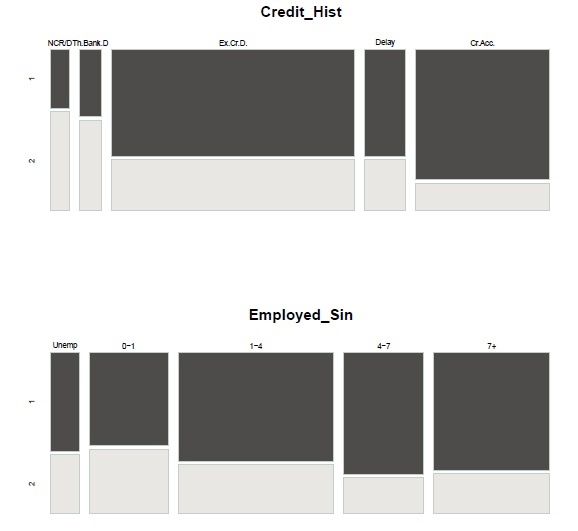
\includegraphics[scale=0.4]{Figures/mosaic_final}
	\end{center}
\end{figure}
\begin{itemize}
\end{itemize}
}


%%%%%%%%%%%%%%%%%%%%%%%%%%%%%%%%%%%%%%%%%%%%%%%%%%%%%%%%%%%%%%%%%%%%%%%%%%%%%%%%%%%%%%%%%%%%%%%%%%%%%%%%%%%%%%%%%%%%%%%%

\frame{
\frametitle{Histogram}
\begin{figure}[htb]
	\begin{center}
	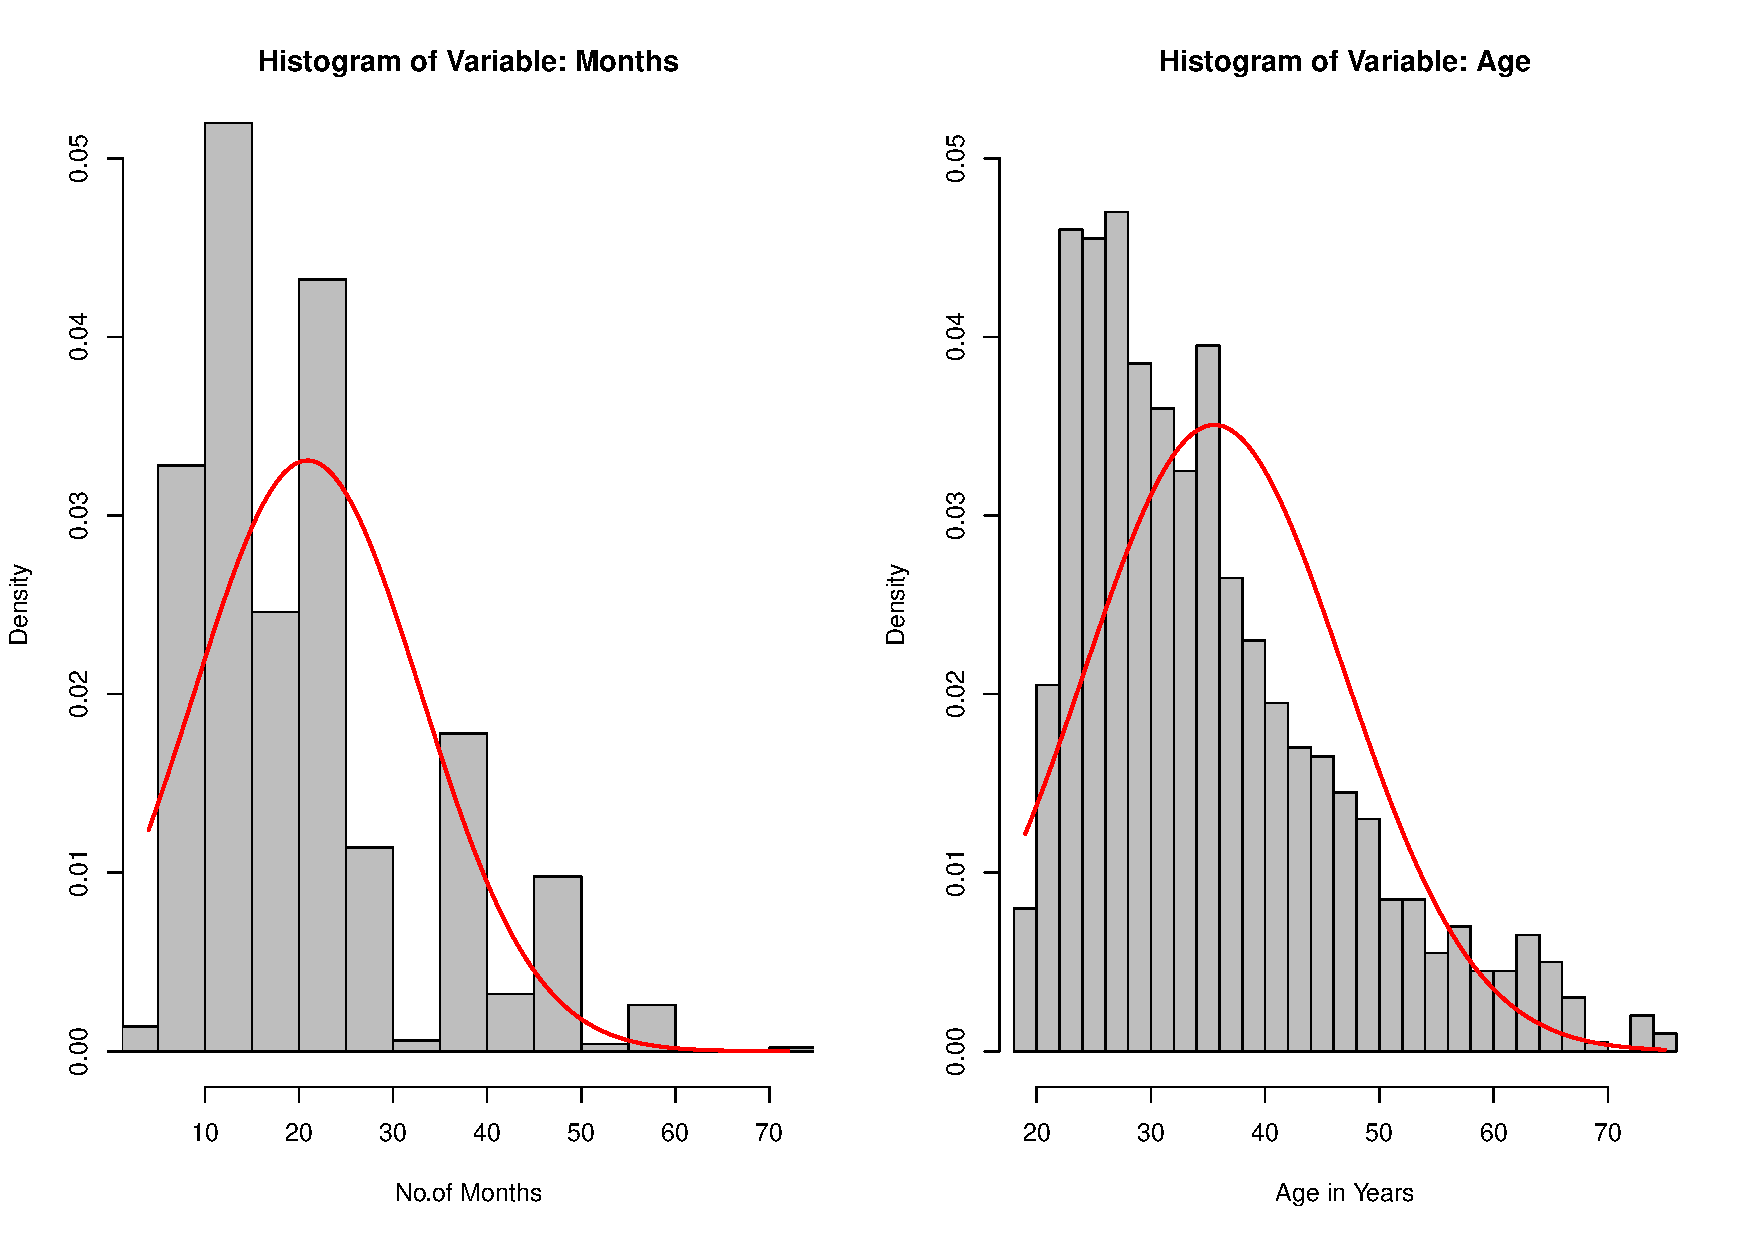
\includegraphics[scale=0.25]{Figures/hist_final}
	\end{center}
\end{figure}
\begin{itemize}
\item Superimposed with Normal Distribution
\end{itemize}
}

%%%%%%%%%%%%%%%%%%%%%%%%%%%%%%%%%%%%%%%%%%%%%%%%%%%%%%%%%%%%%%%%%%%%%%%%%%%%%%%%%%%%%%%%%%%%%%%%%%%%%%%%%%%%%%%%%%%%%%%%

\frame{
\frametitle{Kernel Density}
\begin{figure}[htb]
	\begin{center}
	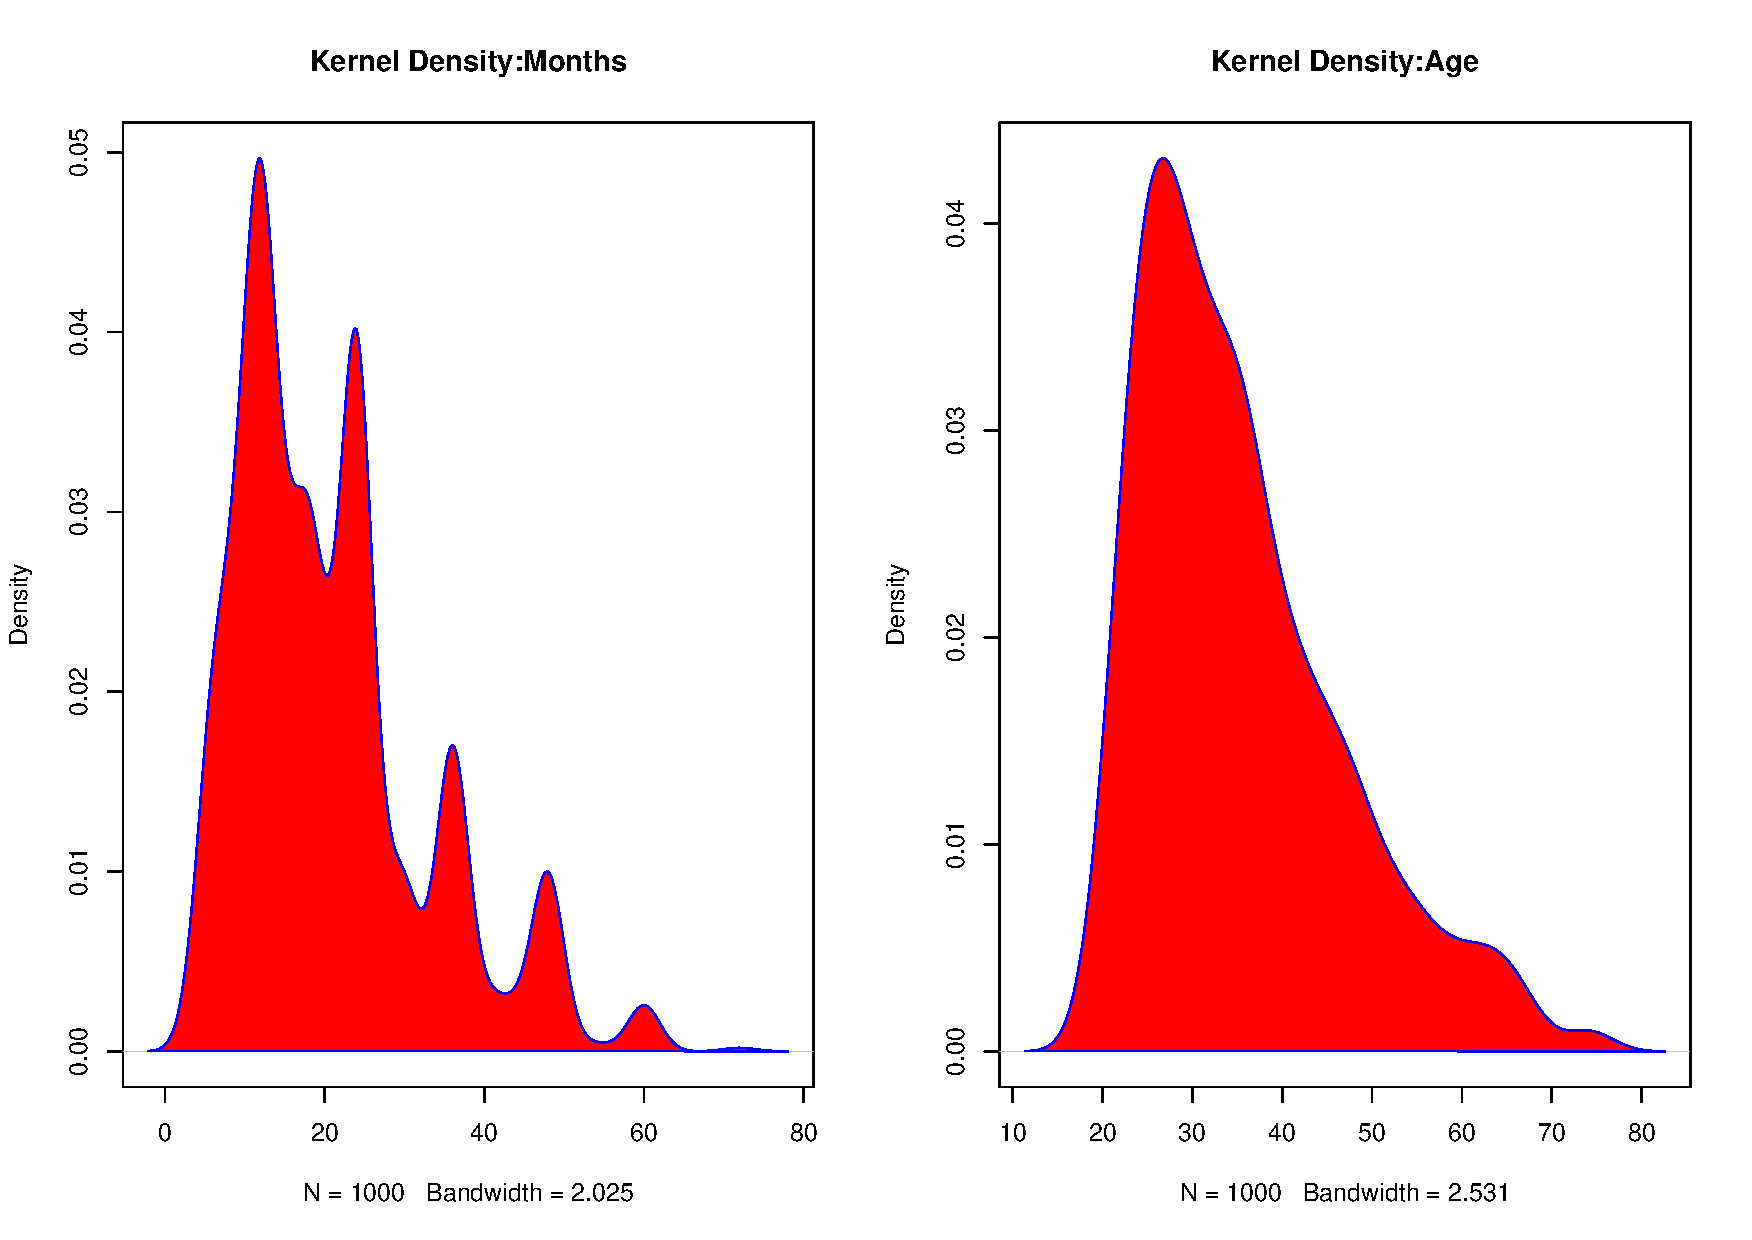
\includegraphics[scale=0.25]{Figures/kernel_final}
	\end{center}
\end{figure}
\begin{itemize}
\item Accurate measure of probability density 

\end{itemize}
}

%%%%%%%%%%%%%%%%%%%%%%%%%%%%%%%%%%%%%%%%%%%%%%%%%%%%%%%%%%%%%%%%%%%%%%%%%%%%%%%%%%%%%%%%%%%%%%%%%%%%%%%%%%%%%%%%%%%%%%%%

\frame{
\frametitle{Box Plots}
\begin{figure}[htb]
	\begin{center}
	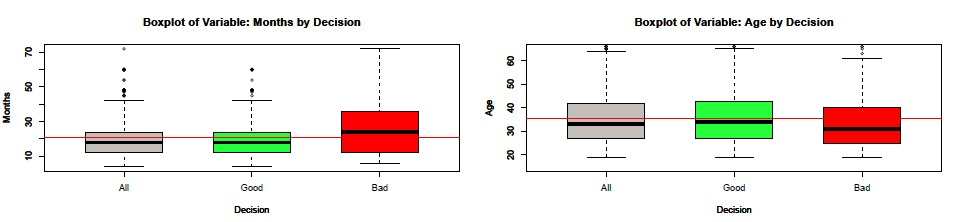
\includegraphics[scale=0.45]{Figures/boxplot_final}
	\end{center}
\end{figure}
\begin{itemize}
\item Outlier detection
\end{itemize}
}

\section{Data Manipulation}
%%%%%%%%%%%%%%%%%%%%%%%%%%%%%%%%%%%%%%%%%%%%%%%%%%%%%%%%%%%%%%%%%%%%%%%%%%%%%%%%%%%%%%%%%%%%%%%%%%%%%%%%%%%%%%%%%%%%%%%%
\frame{
\frametitle{Encoding Data}
\begin{itemize}
\item Real world data-set usually contains two types of predictors
	\begin{itemize}
	\item Categorical
	\item Continuous
	\end{itemize}
\item We performed industry-wide used transformations on these predictors	
\end{itemize}
}
%%%%%%%%%%%%%%%%%%%%%%%%%%%%%%%%%%%%%%%%%%%%%%%%%%%%%%%%%%%%%%%%%%%%%%%%%%%%%%%%%%%%%%%%%%%%%%%%%%%%%%%%%%%%%%%%%%%%%%%%

\frame[containsverbatim]{
\frametitle{Encoding Categorical Data}
\begin{itemize}
\item Dummy encoding transformation was applied to transform them into numerical forms.
\begin{lstlisting}
dummies = dummyVars( ~ ., data = dat_cat[,1:(ncol(dat_cat)-2)])
category_data_dummies=as.data.frame(predict(dummies,newdata=dat_cat[,1:(ncol(dat_cat)-2)]))
\end{lstlisting}		
\end{itemize}
}


\frame[containsverbatim]{
\frametitle{Encoding Continuous Data}
\begin{itemize}
\item We performed outlier detection and imputation by replacing values with z value higher than 3 with predictor's mean value
\item Outlier Function:
\begin{lstlisting}
remove_outliers = function(x, na.rm = TRUE, ...) 
VarMean = mean(x, na.rm = na.rm, ...)
VarSD = sd(x,na.rm = na.rm, ...)
y = x
y[abs((x - VarMean)/VarSD) >3] = NA
y
\end{lstlisting}
\item We applied this function on dataset using sapply
\item Imputed the NA replacements with mean value.	
\end{itemize}
}


%%%%%%%%%%%%%%%%%%%%%%%%%%%%%%%%%%%%%%%%%%%%%%%%%%%%%%%%%%%%%%%%%%%%%%%%%%%%%%%%%%%%%%%%%%%%%%%%%%%%%%%%%%%%%%%%%%%%%%%%

\frame[containsverbatim]{
\frametitle{Scaling Data}
\begin{itemize}
\item A (-1 to 1) scaling transformation was applied on the data to make them more comprehensible for algorithms
\item Formula:
\begin{lstlisting}
## MinMaxScaling (-1 to 1)
min_max_scaling=function(col)((col-min(col))/(max(col)-min(col))*2-1)
##check
min_max_scaling(c(1,2,3,4))
[1] -1.0000000 -0.3333333  0.3333333  1.0000000
\end{lstlisting}
\item The formula was applied on dataset using sapply	
\end{itemize}
}
%%%%%%%%%%%%%%%%%%%%%%%%%%%%%%%%%%%%%%%%%%%%%%%%%%%%%%%%%%%%%%%%%%%%%%%%%%%%%%%%%%%%%%%%%%%%%%%%%%%%%%%%%%%%%%%%%%%%%%%%


\frame{
\frametitle{Sampling Data}
\begin{itemize}
\item The dataset was randomly divided into Train(60\%), Validation(20\%) and Test samples(20\%) with control over target variable (same distribution of target variable in each sample).
\item We used "createFolds" function of caret package which has similar functionality of dividing data.
\item We removed variables with 0 variances using caret's "nearZeroVar" function and saved the samples sets.	
\end{itemize}
}
%%%%%%%%%%%%%%%%%%%%%%%%%%%%%%%%%%%%%%%%%%%%%%%%%%%%%%%%%%%%%%%%%%%%%%%%%%%%%%%%%%%%%%%%%%%%%%%%%%%%%%%%%%%%%%%%%%%%%%%%
\frame[containsverbatim]{
\frametitle{Sampling Data}
\begin{lstlisting}
library(caret)
set.seed(3456)
##dividing rows in 5 folds with control over target variable 

devIndex = as.data.frame(createFolds(data_final$dv, k=5,  list = TRUE))

data_div_1= data_final[devIndex$Fold1,c("id","dv")]
data_div_2= data_final[devIndex$Fold2,c("id","dv")]
data_div_3= data_final[devIndex$Fold3,c("id","dv")]
data_div_4= data_final[devIndex$Fold4,c("id","dv")]
data_div_5= data_final[devIndex$Fold5,c("id","dv")]

\end{lstlisting}	
}
\section{Predictive Modelling}
%%%%%%%%%%%%%%%%%%%%%%%%%%%%%%%%%%%%%%%%%%%%%%%%%%%%%%%%%%%%%%%%%%%%%%%%%%%%%%%%%%%%%%%%%%%%%%%%%%%%%%%%%%%%%%%%%%%%%%%%

\frame{
\frametitle{Methodology}
\begin{figure}[htb]
	\begin{center}
	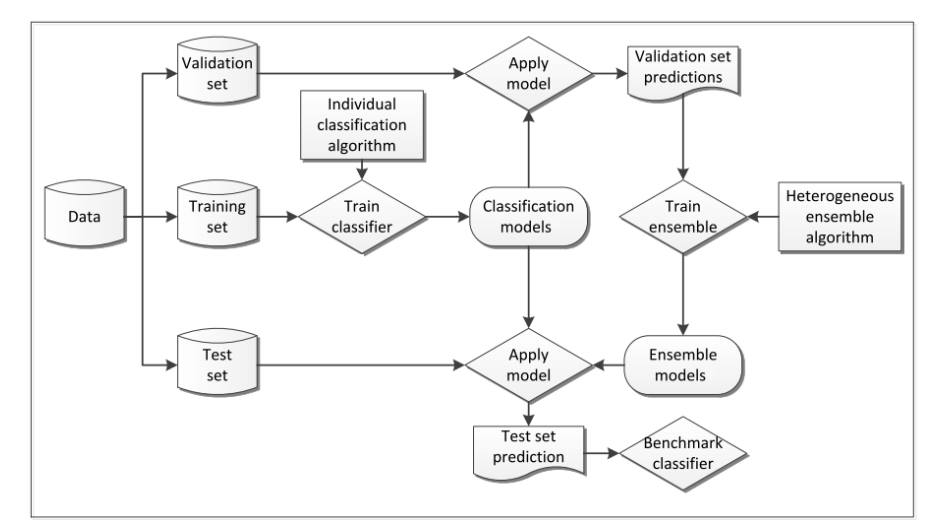
\includegraphics[scale=0.275]{Figures/predictive_methodology}
	\caption{Schematic View of Predictive Modelling Process}
	\end{center}
\end{figure}
}

%Our Objective
%Step 1  Following a careful approach to minimize forced errors, we will %pre-process the dataset and make sub-samples of training data.
%Step 2  We will build a model library with diverse set of classiers and varying parametric values.
%Step 3  Apply Stacking Ensemble method and compare results with individual algorithms.

%%%%%%%%%%%%%%%%%%%%%%%%%%%%%%%%%%%%%%%%%%%%%%%%%%%%%%%%%%%%%%%%%%%%%%%%%%%%%%%%%%%%%%%%%%%%%%%%%%%%%%%%%%%%%%%%%%%%%%%%

\frame{
\frametitle{Sub-sampling using cross validation}
\begin{itemize}
\item To increase diversity for ensemble modelling, we applied cross validation method, except the validation part.
\item Created 5 folds out of Training dataset with control over target variable.
	\begin{center}
	\includegraphics[scale=0.3]{Figures/3_K-fold}
	\end{center}
\end{itemize}
}

%%%%%%%%%%%%%%%%%%%%%%%%%%%%%%%%%%%%%%%%%%%%%%%%%%%%%%%%%%%%%%%%%%%%%%%
\frame{
\frametitle{Further Sampling using Bootstrap Aggregation (Bagging)}
\begin{itemize}
\item Bagging is random selection from original dataset with replacements.
\item We controlled the random selection to 67-70 percent being the original data.
	\begin{center}
	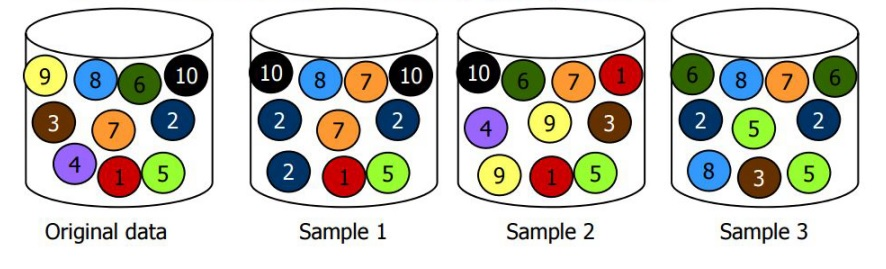
\includegraphics[scale=0.25]{Figures/3_bagging}
	\end{center}
\end{itemize}
}

%%%%%%%%%%%%%%%%%%%%%%%%%%%%%%%%%%%%%%%%%%%%%%%%%%%%%%%%%%%%%%%%%%%%%%%%%%%%%%%%%%%%%%%%%%%%%%%%%%%%%%%%%%%%%%%%%%%%%%%%

\frame{
\frametitle{Sub Sampling Overview}
\begin{itemize}
	\begin{center}
	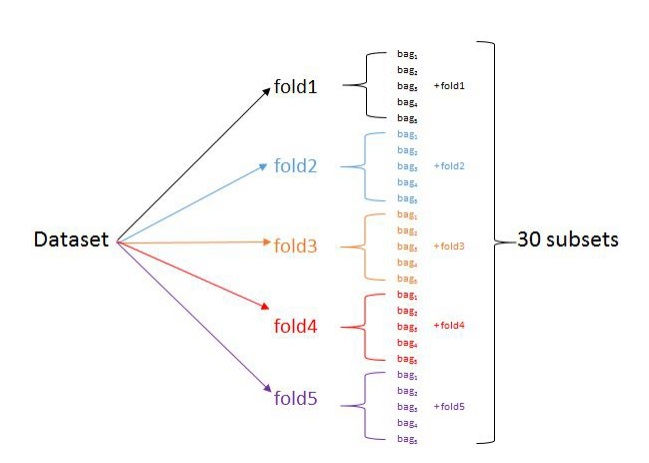
\includegraphics[scale=0.5]{Figures/3_Sample_Chart}
	\end{center}
\end{itemize}
}

%%%%%%%%%%%%%%%%%%%%%%%%%%%%%%%%%%%%%%%%%%%%%%%%%%%%%%%%%%%%%%%%%%%%%%%%%%%%%%%%%%%%%%%%%%%%%%%%%%%%%%%%%%%%%%%%%%%%%%%%
\frame{
\frametitle{Models}
\begin{itemize}
\item Models Used:
	\begin{itemize}
		\item Logistic Regression
		\item Random Forest
		\item Gradient Boosting
	\end{itemize}  
\item Ensemble learning thrives on data diversity, it was in common interest to used maximal number of parametric combinations.
\item Helped in saving time over finding optimal parameter values which otherwise would have been manual labor. 
\end{itemize}	
}

%%%%%%%%%%%%%%%%%%%%%%%%%%%%%%%%%%%%%%%%%%%%%%%%%%%%%%%%%%%%%%%%%%%%%%%%%%%%%%%%%%%%%%%%%%%%%%%%%%%%%%%%%%%%%%%%%%%%%%%%
\frame{
\frametitle{Models}
\begin{itemize}
\item Grid Diagram
	\begin{center}
	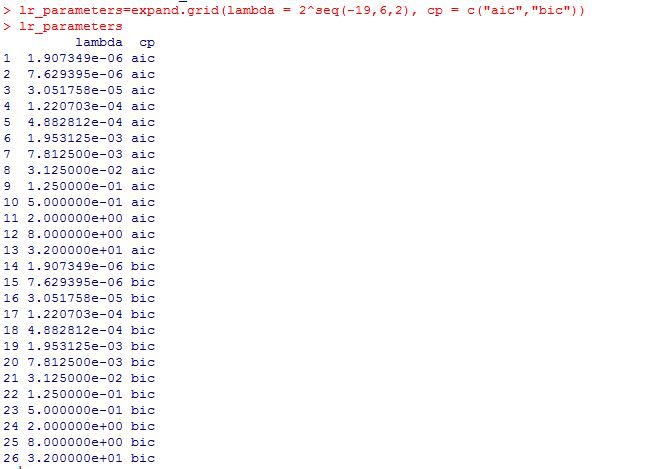
\includegraphics[scale=0.3]{Figures/4_grid}
	\end{center}
	
\item Created models for each sample over all aforementioned parametric values.
\end{itemize}	
}


\frame{
\frametitle{Model}
\begin{itemize}
\item To speed up the process we used "doSNOW" and "foreach" packages which allows parallel processing.
\item Instead of 1 core, we could now engage 3 cores simultaneously for this purpose.
\item For each dataset, a for loop was required to parse through parametric grid.
\end{itemize}
}

%%%%%%%%%%%%%%%%%%%%%%%%%%%%%%%%%%%%%%%%%%%%%%%%%%%%%%%%%%%%%%%%%%%%%%%%%%%%%%%%%%%%%%%%%%%%%%%%%%%%%%%%%%%%%%%%%%%%%%%%

\frame[containsverbatim]{
\frametitle{Models Overview}
\begin{table}
\begin{center}
\begin{tabular}{ccc} 
\hline\hline
Classifier  & No.of Models& No.of Candidates\\ 
\hline
Logistic Regression  & 26 & 780 \\
ANN  & 72 & 2160 \\
Random Forest  & 54 & 1620 \\
Total & 152 & 4560 \\
\hline\hline
\end{tabular}
\caption{Overview of base models}
\end{center}
\end{table}
}



%%%%%%%%%%%%%%%%%%%%%%%%%%%%%%%%%%%%%%%%%%%%%%%%%%%%%%%%%%%%%%%%%%%%%%%%%%%%%%%%%%%%%%%%%%%%%%%%%%%%%%%%%%%%%%%%%%%%%%%%

\frame{
\frametitle{Combining and Cleaning}
\begin{itemize}
\item Combining
	\begin{itemize}
	\item Since the predictions of algorithms were saved in different 			CSVs, we had to combine them for final ensemble learning.
	\item We used "import" and "do.call" function  of plyr package which 	called "read.csv" and "cbind" on all the CSVs in a single line code.
	\end{itemize}
\item Correlation
	\begin{itemize}
	\item Removed candidates with more than 0.85 correlation value with 		other candidates
	\end{itemize}
\end{itemize}
}

\frame[containsverbatim]{
\frametitle{Ensemble Learning and Scoring Results}

\begin{itemize}
\item Ensemble Creation
	\begin{itemize}
	\item We used logistic regression and random forest as generalizer to predict the target 	variable using candidates.
	\end{itemize}
\item Results
	\begin{itemize}
	\item We calculated AUC (Area under the score) value for judging model 
		performances.
	\end{itemize}	

\begin{table}
\begin{center}
\begin{tabular}{cc} 
\hline\hline
Algorithm & AUC value\\ 
\hline
Stacking with RF & 0.812  \\
Stacking with LogR & 0.70 \\
ANN & 0.770 \\
RF & 0.791 \\
LogR & 0.761 \\
\hline\hline
\end{tabular}
\caption{Summary of Performance scores}
\end{center}
\end{table}
\end{lstlisting}
}

\frame{
\begin{center}
Thank You
\end{center}
}
%%%%%%%%%%%%%%%%%%%%%%%%%%%%%%%%%%%%%%%%%%%%%%%%%%%%%%%%%%%%%%%%%%%%%%%%%%%%%%%%%%%%%%%%%%%%%%%%%%%%%%%%%%%%%%%%%%%%%%%%
% Define the end of the document:
\end{document}
